\documentclass[aspectratio=169,usenames,dvipsnames]{beamer}
\usetheme{Pittsburgh}
\usepackage{xcolor}
\usepackage[utf8]{inputenc}
\usepackage[german]{babel}
\usepackage{amsmath}
\usepackage{amsfonts}
\usepackage{amssymb}
\usepackage{graphicx}
\usepackage{multicol}
\usepackage{wrapfig}
\usepackage{hyperref}
\usepackage{tikz}
\usepackage{neuralnetwork}

\usetikzlibrary{shapes,arrows,chains}

\author{Jonas Betzendahl}
\title{Algorithmen und Du}

\beamertemplatenavigationsymbolsempty 

%src: https://tex.stackexchange.com/questions/34921/how-to-overlap-images-in-a-beamer-slide
\def\Put(#1,#2)#3{\leavevmode\makebox(0,0){\put(#1,#2){#3}}}

\begin{document}

%------------------------------------------------------------------------------------
\section{Introduction}

\begin{frame}
\begin{center}
\vfill
\huge Algorithmen und Du
\normalsize 
\smallskip
\smallskip

Warum Künstliche Intelligenz Nie Politisch Neutral Sein Kann
\bigskip\bigskip

\large Jonas Betzendahl, M.Sc.\\\normalsize FAU Erlangen-Nürnberg, KWARC
\bigskip\bigskip\large

\href{https://twitter.com/lambdatotoro}{
\includegraphics[scale=0.125]{images/twitter_logo.png}}
\href{https://chaos.social/@lambdatotoro}{\includegraphics[scale=0.125]{images/mastodon_logo.png}}
\href{https://github.com/lambdaTotoro}{
\includegraphics[scale=0.125]{images/github_logo.png}}

\texttt{@lambdaTotoro (@chaos.social)}
\end{center}
\end{frame}

%------------------------------------------------------------------------------------


\begin{frame}
\begin{center}
\LARGE
Wohin man auch schaut\dots
\bigskip

\Huge
Künstliche Intelligenz\\
ist überall
\end{center}
\end{frame}

\begin{frame}
\frametitle{Menschen sind \emph{sehr} fehlbar...}
\begin{minipage}{0.5\textwidth}
\begin{center}
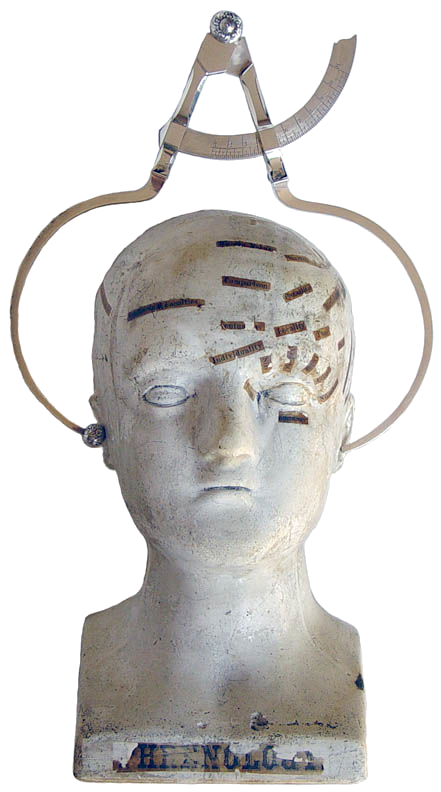
\includegraphics[keepaspectratio, height=0.75\textheight]{images/calipers_transparent}
\end{center}
\end{minipage}\begin{minipage}{0.5\textwidth}
\begin{center}
\pause

\includegraphics[keepaspectratio, height=0.75\textheight]{images/human_bias}
\end{center}
\end{minipage}
\end{frame}

{
    \usebackgroundtemplate{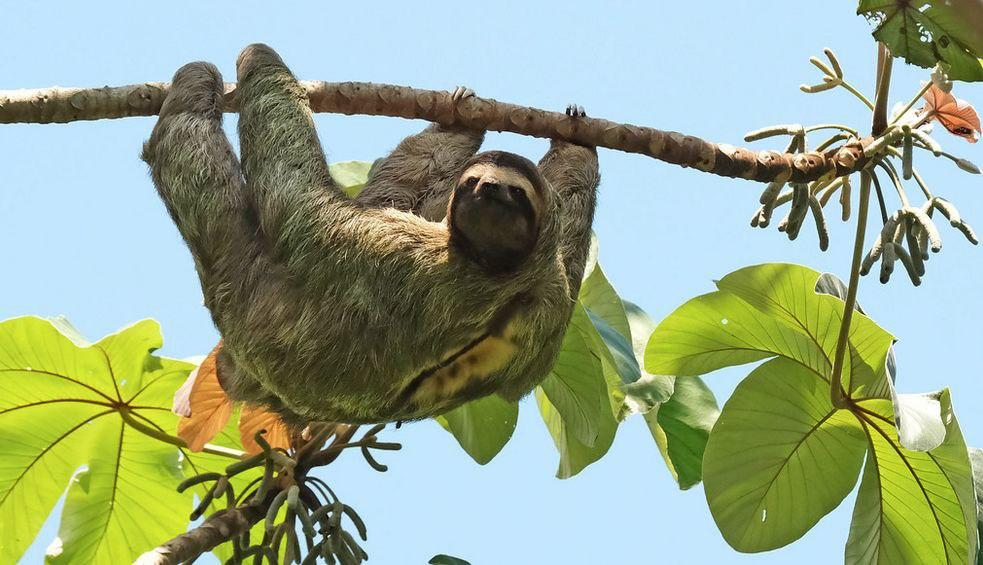
\includegraphics[height=\paperheight,width=\paperwidth]{images/sloth}}
    \setbeamertemplate{navigation symbols}{}
    \begin{frame}[plain]
    \Put(150,170){\color{black}\huge \rotatebox{-10}{...und \emph{sehr} langsam!}}
    \end{frame}
}

{
    \usebackgroundtemplate{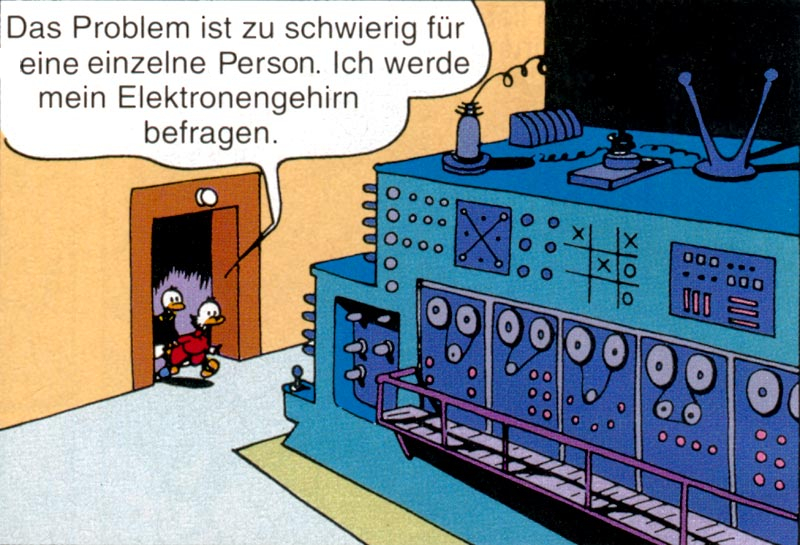
\includegraphics[height=\paperheight,width=\paperwidth]{images/elektronengehirn}}

\begin{frame}

\end{frame}
}
%------------------------------------------------------------------------------------

\section{How it works and weaknesses}

\begin{frame}
\begin{center}
\Huge
Algorithmen \&\\
Maschinelles Lernen
\bigskip

\LARGE
Was ist das? Wie geht das?\\ Und was sind die Probleme?
\end{center}
\end{frame}

\begin{frame}
\begin{center}
\includegraphics[height=0.8\textheight, keepaspectratio]{images/man-cooking-clipart}
\Put(-230,270){\includegraphics[scale=0.05, keepaspectratio,angle=15]{images/arrow}}
\Put(-275,325){\huge Algorithmen}
\end{center}
\end{frame}

{
    \usebackgroundtemplate{
\includegraphics[height=\paperheight,width=\paperwidth]{images/funnel}}
    \setbeamertemplate{navigation symbols}{}
    \begin{frame}[plain]
    \end{frame}
}

\begin{frame}
\begin{minipage}{0.48\textwidth}
\begin{center}
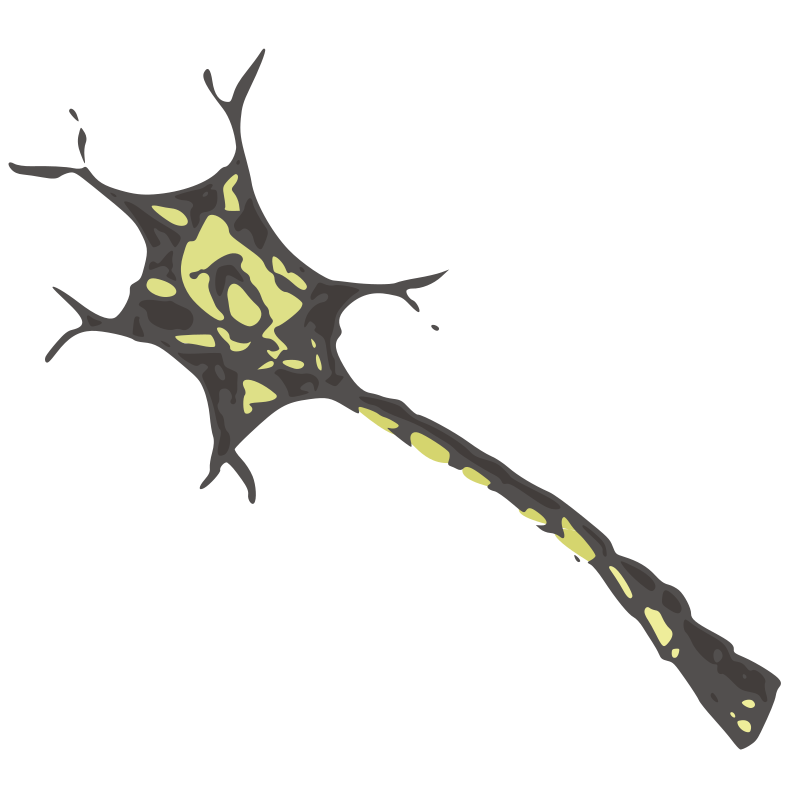
\includegraphics[width=0.8\textwidth, keepaspectratio]{images/neuron} 
\end{center}
\end{minipage}\pause\begin{minipage}{0.48\textwidth}
\begin{center}
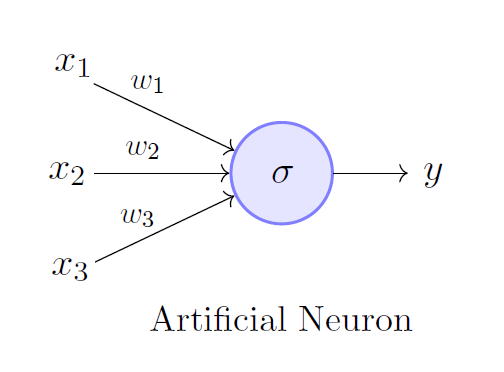
\includegraphics[width=0.99\textwidth, keepaspectratio]{images/perceptron} 
\end{center}
\end{minipage}
\end{frame}


{
    \begin{frame}[fragile]
    \begin{center}
    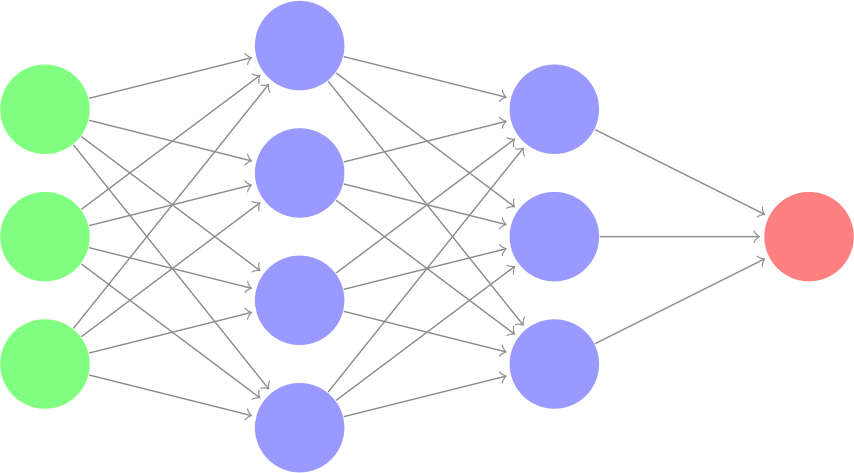
\includegraphics[scale=0.275]{images/neuralnet_white.png} 
    \end{center}
    \pause
    \Put(-10,175){
\includegraphics[width=0.2\textwidth, keepaspectratio]{images/sunflower}}
    \pause
    \Put(315,190){
\includegraphics[width=0.1\textwidth, keepaspectratio]{images/thumbs-up}}
    \end{frame}
}

{
	\setbeamercolor{background canvas}{bg=LimeGreen}
    \begin{frame}[fragile]
    \begin{center}
    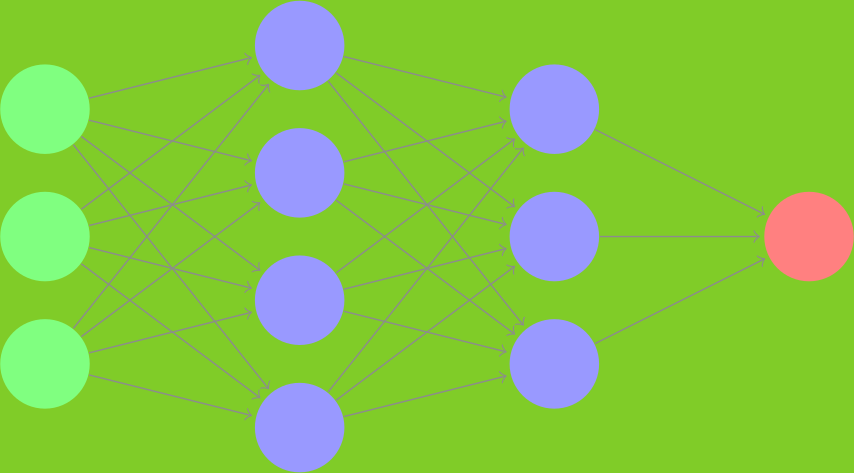
\includegraphics[scale=0.275]{images/neuralnet_green.png} 
    \end{center}
    \Put(-10,175){
\includegraphics[width=0.2\textwidth, keepaspectratio]{images/sunflower}}
    \Put(315,190){
\includegraphics[width=0.1\textwidth, keepaspectratio]{images/thumbs-up}}
    \end{frame}
}


{
    \begin{frame}[fragile]
    \begin{center}
    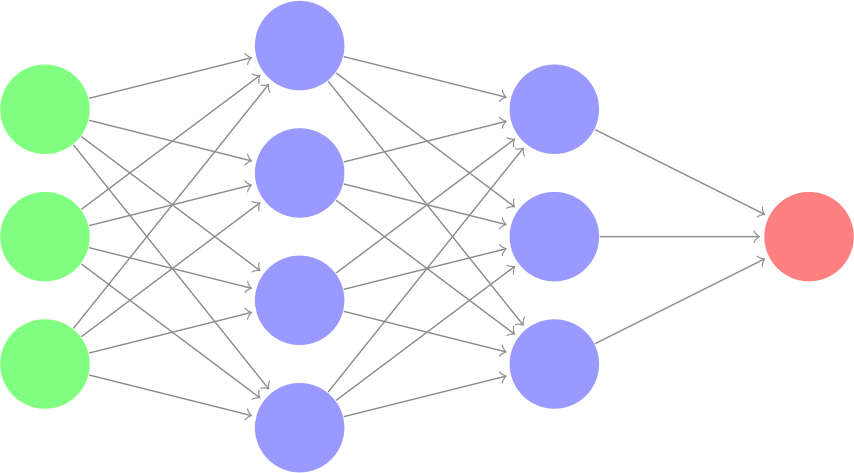
\includegraphics[scale=0.275]{images/neuralnet_white.png} 
    \end{center}
    \pause
    \Put(-10,175){
\includegraphics[width=0.2\textwidth, keepaspectratio]{images/kangaroo}}
    \pause
    \Put(315,160){
\includegraphics[width=0.1\textwidth, keepaspectratio]{images/thumbs-down}}
    \end{frame}
}


{
	\setbeamercolor{background canvas}{bg=LimeGreen}
    \begin{frame}[fragile]
    \begin{center}
    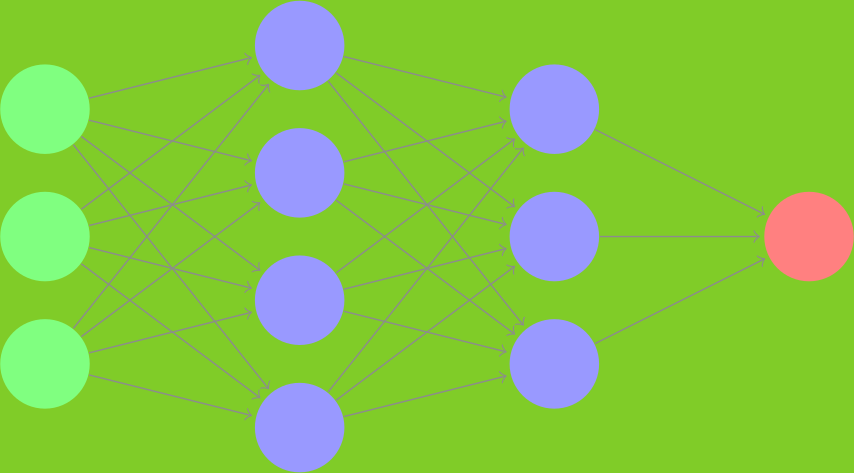
\includegraphics[scale=0.275]{images/neuralnet_green.png} 
    \end{center}
    \Put(-10,175){
\includegraphics[width=0.2\textwidth, keepaspectratio]{images/kangaroo}}
    \Put(315,160){
\includegraphics[width=0.1\textwidth, keepaspectratio]{images/thumbs-down}}
    \end{frame}
}

{
    \begin{frame}[fragile]
    \begin{center}
    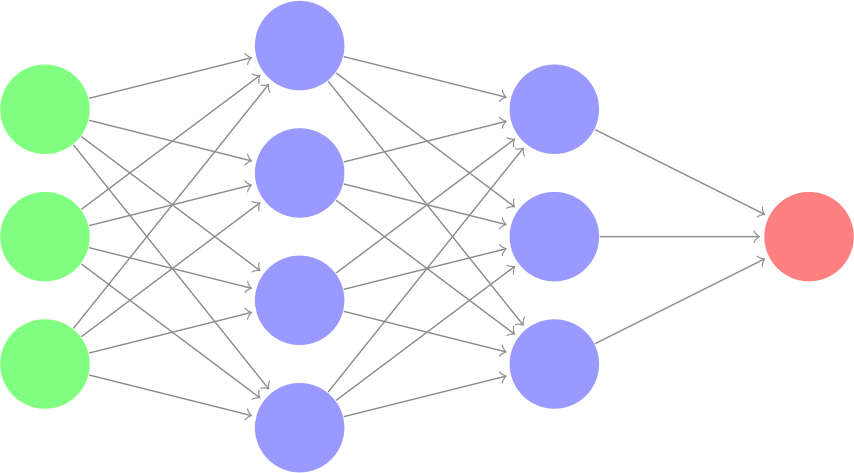
\includegraphics[scale=0.275]{images/neuralnet_white.png} 
    \end{center}
    \pause
    \Put(-10,175){
\includegraphics[width=0.2\textwidth, keepaspectratio]{images/sunflower}}
    \pause
    \Put(315,160){
\includegraphics[width=0.1\textwidth, keepaspectratio]{images/thumbs-down}}
    \end{frame}
}


{
\setbeamercolor{background canvas}{bg=OrangeRed}
    \begin{frame}[fragile]
    \begin{center}
    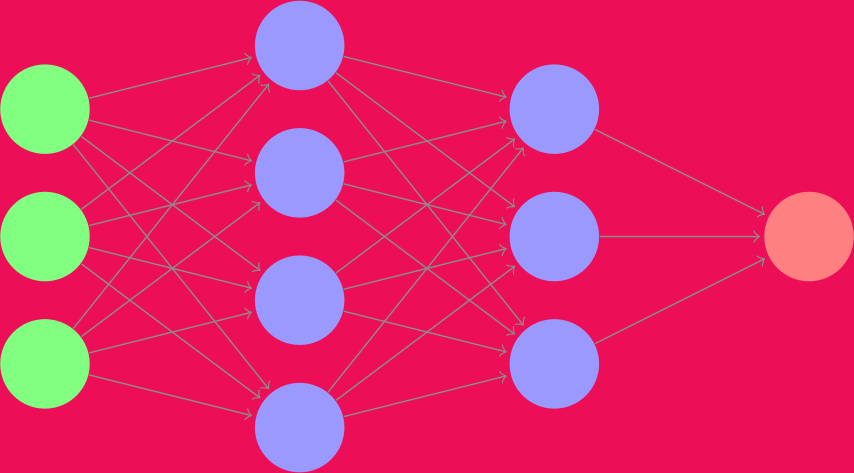
\includegraphics[scale=0.275]{images/neuralnet_red.png} 
    \end{center}
    \Put(-10,175){
\includegraphics[width=0.2\textwidth, keepaspectratio]{images/sunflower}}
    \Put(315,160){
\includegraphics[width=0.1\textwidth, keepaspectratio]{images/thumbs-down}}
    \end{frame}
}

{
    \begin{frame}[fragile]
    \begin{center}
    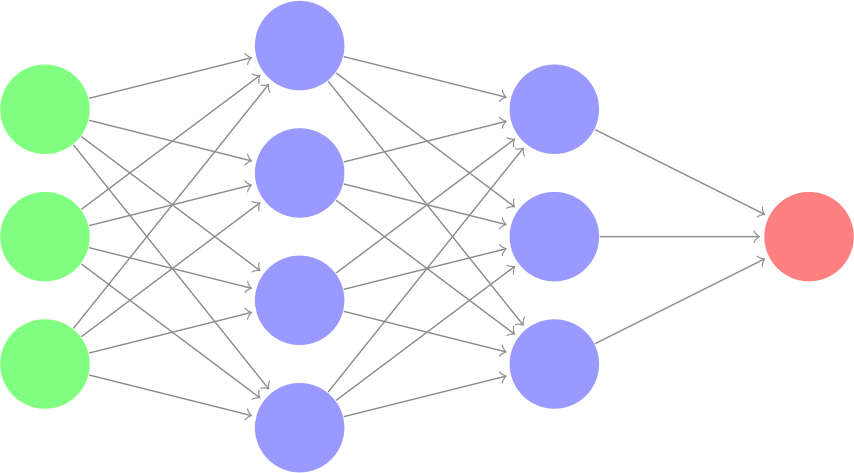
\includegraphics[scale=0.275]{images/neuralnet_white.png} 
    \end{center}
    \Put(-10,175){
\includegraphics[width=0.2\textwidth, keepaspectratio]{images/sunflower}}
    \Put(315,190){
\includegraphics[width=0.1\textwidth, keepaspectratio]{images/thumbs-up}}
    \end{frame}
}

{
    \begin{frame}[fragile]
    \begin{center}
    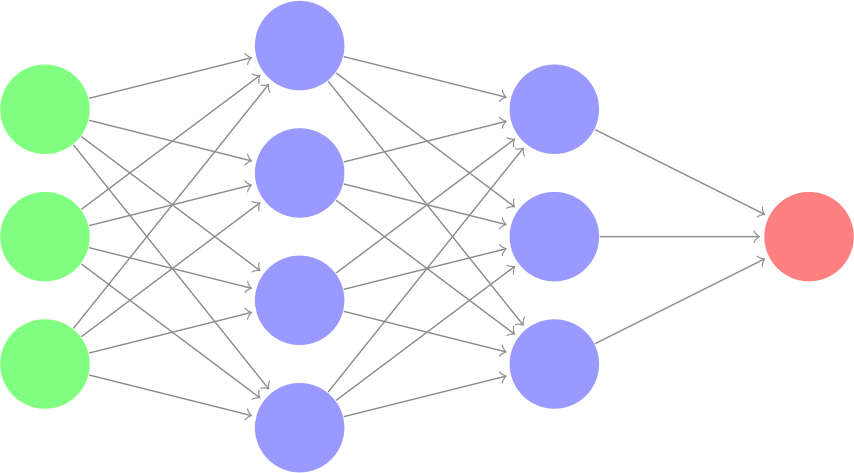
\includegraphics[scale=0.275]{images/neuralnet_white.png} 
    \end{center}
    \Put(-10,175){
\includegraphics[width=0.2\textwidth, keepaspectratio]{images/sunflower_1}}
    \Put(315,190){
\includegraphics[width=0.1\textwidth, keepaspectratio]{images/thumbs-up}}
    \end{frame}
}

\begin{frame}[fragile]
\frametitle{Beeindruckende Mathematik}

\begin{minipage}{0.52\textwidth}
\begin{center}
\includegraphics[scale=0.3]{images/linear_nonlinear.png} 
\end{center}
\end{minipage}\begin{minipage}{0.35\textwidth}
$$y_k = \varphi\left(\sum_{j=0}^m w_{kj}x_j\right)$$
\end{minipage}

\small
\begin{minipage}{0.47\textwidth}
$$\Delta w_{ij}=-\eta \frac{\partial E}{\partial w_{ij}} = -\eta o_i \delta_j$$
$$\lambda(x) = C(t-x)^2$$
$$r_i \dot{y_i} = -y_i \sum_{j=1}^n w_{ji}\sigma\left(y_j - \Theta_j\right) * I_i(t)$$
\end{minipage}\begin{minipage}{0.47\textwidth}
\begin{center}
\includegraphics[scale=0.35]{images/recursive.jpg} 
\end{center}
\end{minipage}
\end{frame}

{
    \usebackgroundtemplate{\includegraphics[height=\paperheight,width=\paperwidth]{images/chain}}
    \begin{frame}
    \Put(0,125){\Huge\emph{Was} wird gelernt?}
    \Put(175,-175){\Huge\emph{Woraus} wird gelernt?}
    \end{frame}
}


%------------------------------------------------------------------------------------

\section{Surely nobody would be this stupid?}

\begin{frame}
\begin{center}
\Huge
KI in der freien Wildbahn
\bigskip

\Large
Leider nicht nur theoretisch problematisch\dots
\end{center}
\end{frame}

\begin{frame}
\begin{minipage}{.5\textwidth}
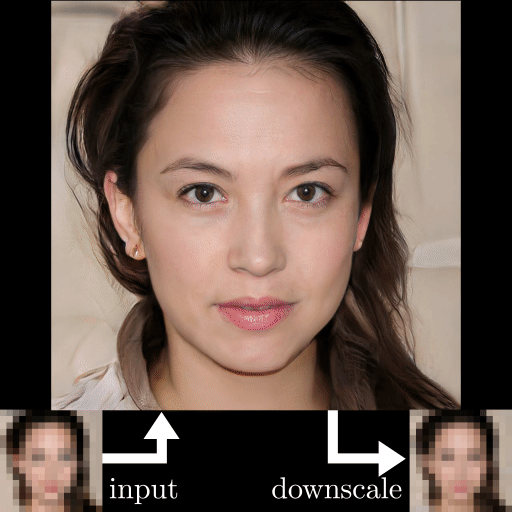
\includegraphics[width=0.9\textwidth, keepaspectratio]{images/step13}
\end{minipage}\begin{minipage}{.5\textwidth}
\textbf{De-pixel-iser}
\bigskip

Wäre es nicht toll, wenn wir aus einem stark verpixelten Foto raten könnten, wie eine Person aussieht, wie bei CSI?
\bigskip

``Computer! Enhance!''
\end{minipage}
\end{frame}

\begin{frame}
\begin{center}
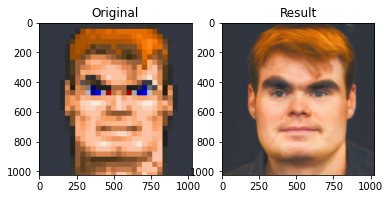
\includegraphics[scale=1]{images/doomguy} 
\end{center}
\end{frame}

\begin{frame}
\begin{center}
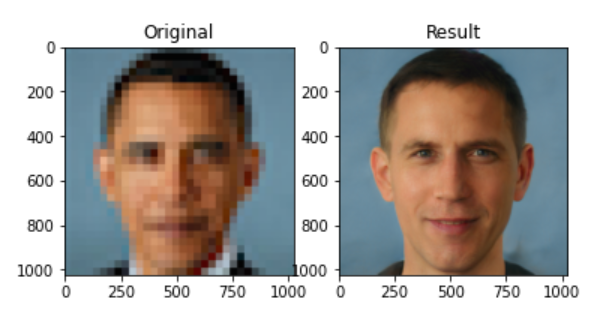
\includegraphics[scale=0.9]{images/obama} 
\end{center}
\pause
\Put(-75,400){\includegraphics[scale=2.7, angle=-15]{images/falsch_gelernt} }
\end{frame}

\begin{frame}
\begin{center}
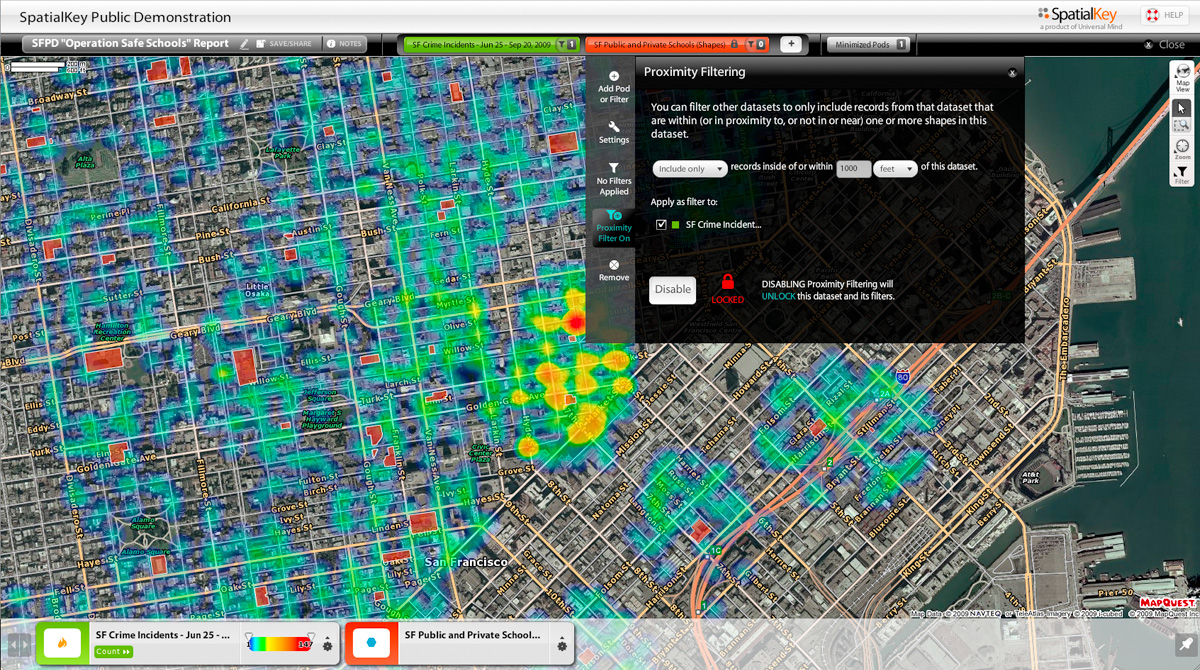
\includegraphics[height=0.8\textheight, keepaspectratio]{images/predictive_policing} 
\end{center}
\pause
\Put(-75,250){\includegraphics[scale=2.7, angle=12]{images/falsch_gelernt} }
\end{frame}

\begin{frame}
\frametitle{Konsequenzen am Arbeitsmarkt}
\begin{minipage}{.5\textwidth}
\begin{center}
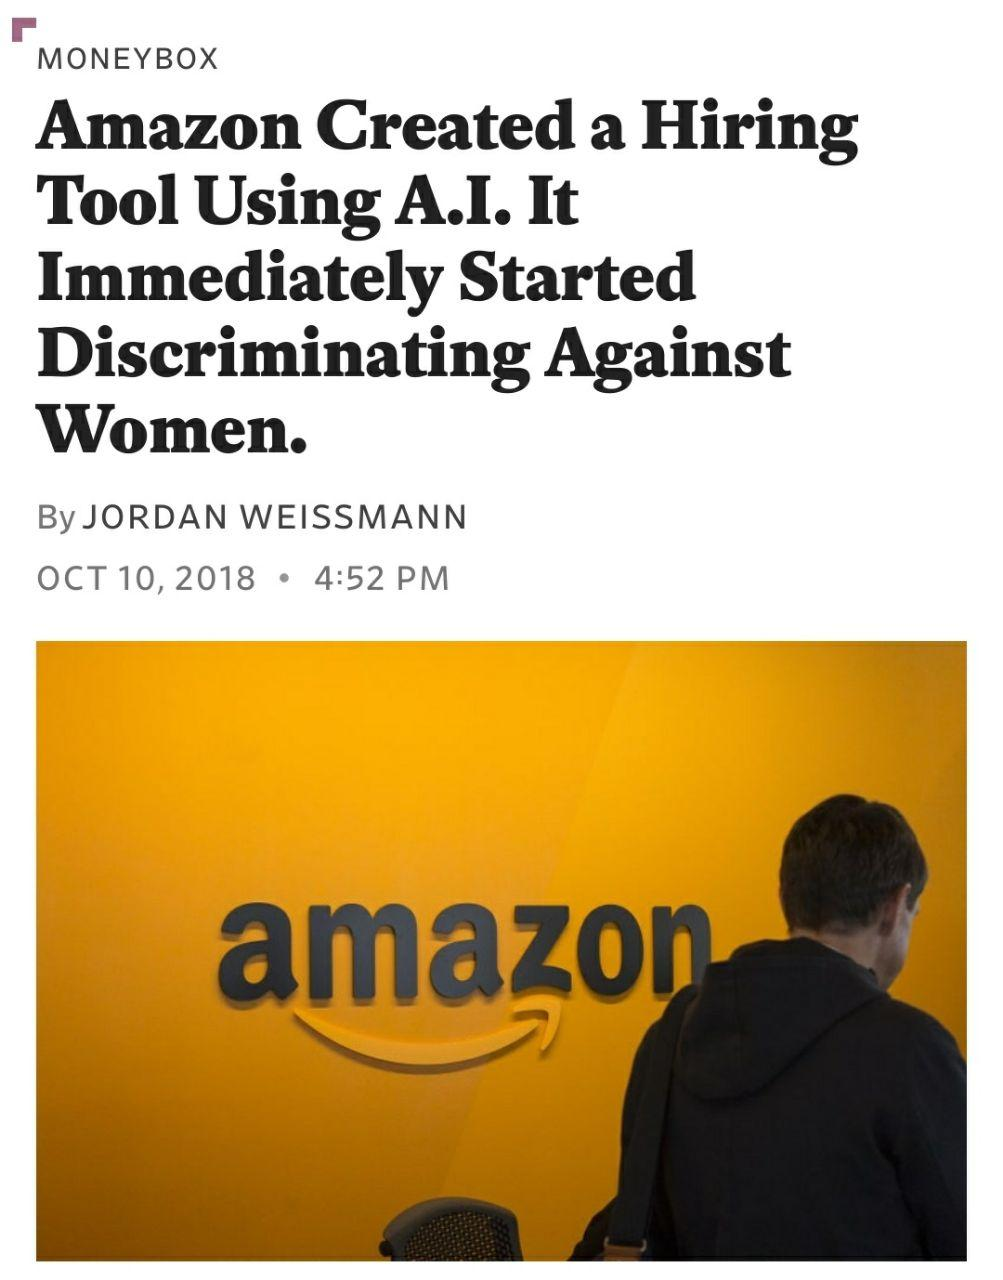
\includegraphics[height=0.75\textheight, keepaspectratio]{images/amazon_hiring}
\end{center}
\end{minipage}\begin{minipage}{.5\textwidth}
\begin{center}
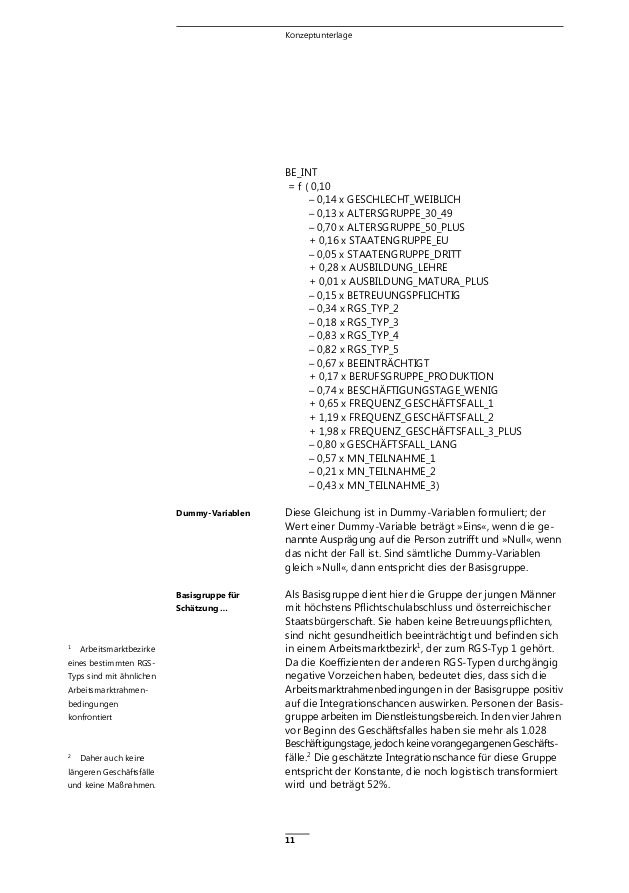
\includegraphics[height=0.75\textheight, keepaspectratio]{images/negativfaktor}
\end{center}
\end{minipage}

\pause
\Put(-40,200){\includegraphics[scale=2.3, angle=15]{images/konsequenzen_ignoriert.png} }
\end{frame}
\begin{frame}

\begin{center}

\includegraphics[width=\textwidth, keepaspectratio]{images/trustworthiness_tweet}
\end{center}

\end{frame}

\begin{frame}

\begin{center}
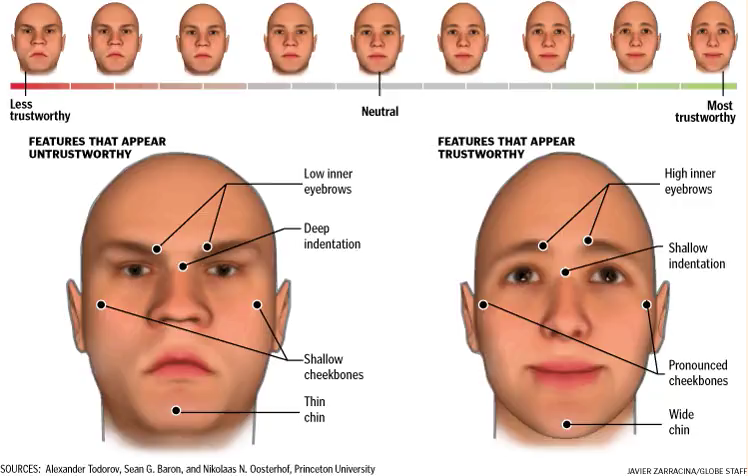
\includegraphics[height=0.95\textheight, keepaspectratio]{images/trustworthiness}
\pause

\Put(-175,270){\includegraphics[scale=1.15, angle=-5]{images/phrenology_bad}}
\pause

\Put(20,290){\includegraphics[scale=1.1, angle=5]{images/phrenology_good}}
\end{center}

\end{frame}

{
    \usebackgroundtemplate{\includegraphics[height=\paperheight,width=\paperwidth]{images/thomas}}
    \setbeamertemplate{navigation symbols}{}
    \begin{frame}[plain]
    \end{frame}
}

%------------------------------------------------------------------------------------

\section{What to do about it?}

\begin{frame}
\begin{center}
\huge
Was tun wir dagegen?

\large
take-home messages
\normalsize
\end{center}
\bigskip

Jedes Mal wenn \glqq Künstliche Intelligenz\grqq\ oder \glqq Maschinelles Lernen\grqq\ aufkommen:
\medskip

\begin{itemize}
\item \emph{Woher} wird gelernt? Welches \emph{Datenset} wird benutzt?
\item \emph{Was} wird gelernt? Worauf wird \emph{optimiert}?
\item Was sind die \emph{Folgen} von diesen Entscheidungen?
\item Haben wir eine Möglichkeit, \emph{Menschen} entscheiden zu lassen?
\end{itemize}

\pause\bigskip\bigskip
\begin{center}
\large
skeptisch bleiben!
\end{center}
\Put(265,45){\includegraphics[scale=0.5, keepaspectratio]{images/thinking_emoji}}
\end{frame}

%------------------------------------------------------------------------------------

\begin{frame}
\frametitle{Quellen:}
\scriptsize
\begin{itemize}
\item Diskriminierung b. Wohnungssuche ``Hanna und Ismail'', Köppen et al.  2017\\
\url{https://www.hanna-und-ismail.de/}

\item ``Amazon Created a Hiring Tool Using A.I. It Immediately Started Discriminating Against Women.'', Weissmann, 2018\\ \url{https://slate.com/business/2018/10/amazon-artificial-intelligence-hiring-discrimination-women.html}

\item ``Machine Bias'', Angwin et al., ProPublica, 2016\\ \url{https://www.propublica.org/article/machine-bias-risk-assessments-in-criminal-sentencing}

\item ``Negativfaktor Frau'', Ingrid Brodnig, 2018 \\ \url{www.profil.at/meinung/ingrid-brodnig-negativfaktor-frau-10422551}

\item ``AI used for first time in job interviews in UK to find best applicants'', The Telegraph, 2019-09-27 \\ \url{https://www.telegraph.co.uk/news/2019/09/27/ai-facial-recognition-used-first-time-job-interviews-uk-find/}

\item ``Predictive policing algorithms are racist. They need to be dismantled.'', MIT Technology Review, 2020-07-17 \\ \url{https://www.technologyreview.com/2020/07/17/1005396/predictive-policing-algorithms-racist-dismantled-machine-learning-bias-criminal-justice/}

\end{itemize}
\end{frame}
\end{document}

